\newpage 
\section{Tip Convolution for Hard Sphere Model \label{Appendix: Tip Convolution for Hard Sphere Model}}

From geometry:
\begin{equation}
cos(\alpha) = \frac{X_{tip}}{R_{surface}+R_{tip} }
\end{equation}

\begin{equation}
sin(\alpha) = \frac{Z_{tip}+R_{tip}}{R_{surface}+R_{tip}} \end{equation}


From trigonomerty:
\begin{equation}
sin(\alpha) = \frac{\sqrt{(R_{surface}+R_{tip})^2-X_{tip}^2}}{R_{surface}+R_{tip} }
\end{equation}

Therefore:
\begin{equation} \frac{\sqrt{(R_{surface}+R_{tip})^2-X_{tip}^2}}{R_{surface}+R_{tip}} = \frac{Z_{tip}+R_{tip}}{R_{surface}+R_{tip}} 
\end{equation}

\begin{equation}
Z_{tip} = \sqrt{(R_{surface}+R_{tip})^2-X_{tip}^2} - R_{tip}
\end{equation}

\begin{figure}[H]
    \centering
    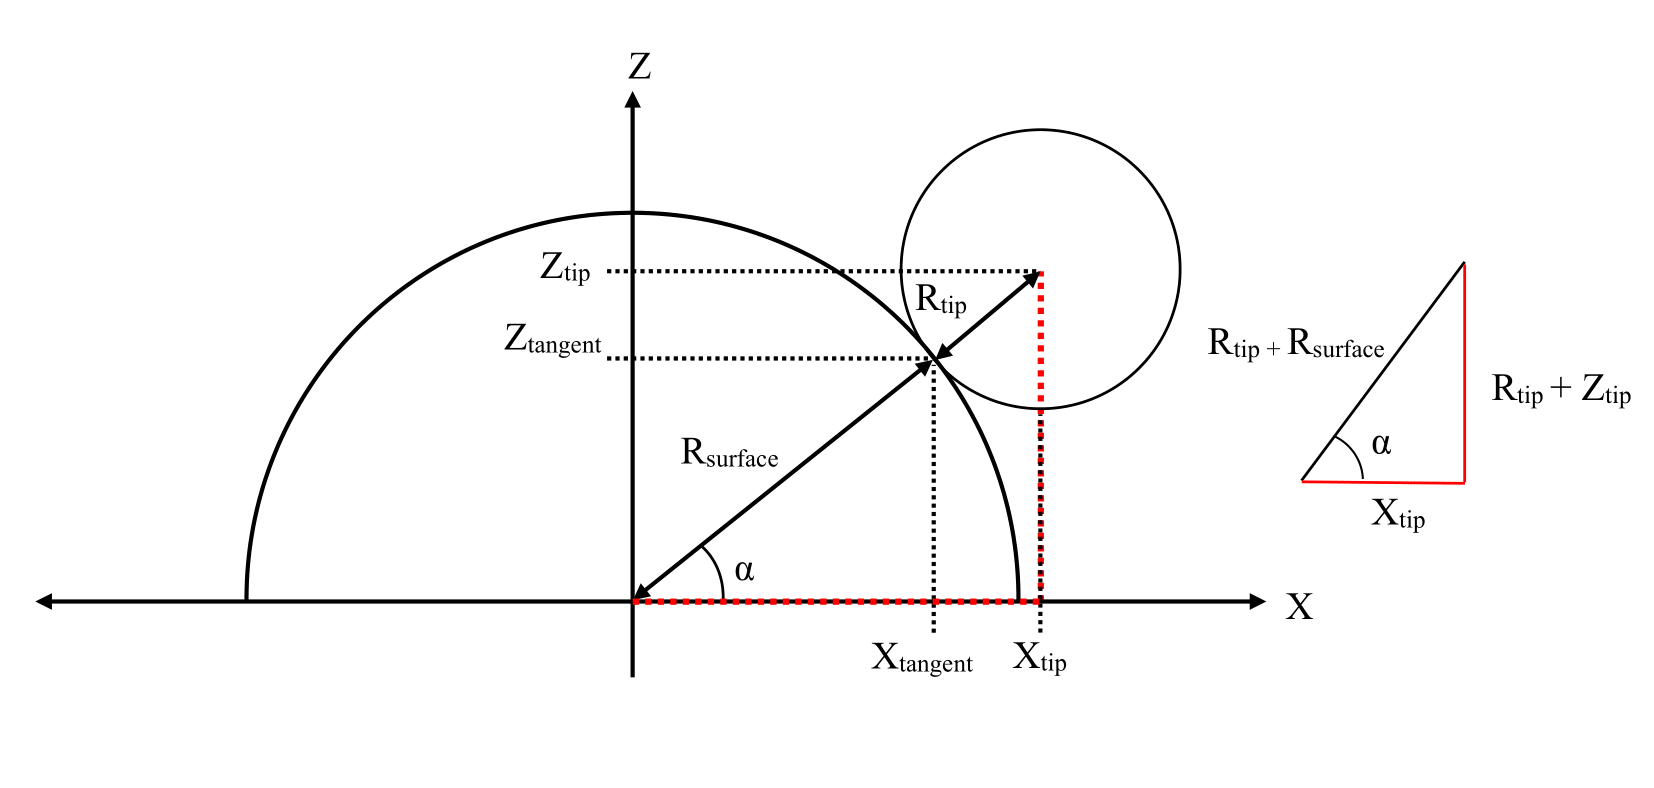
\includegraphics[width=1\linewidth]{Figures/TipConvolution Diagram-1.png}
    \caption{\label{fig: TipConvolution Diagram} Example two dimensional heat map of indentation force over the scanning axis for semi-sphere structure. Including overlayed contour of constant force }
\end{figure}